%\inputencoding{utf8}

\section{Solution}
The idea behind categorization-based concept arises from general requirements categorization and goes ahead with the arrangement of requirements in formal structure categorizing them by their characteristics and thereby, forming an attached combination of the categories (\textit{aspects}). This combination of \textit{aspects} reflects a structure of the requirements scope and constitutes a new Artifact. 

For better explanation of categorization-based concept, a use case of \textit{aspects} utilization for structuring textual requirements implemented in AutoFOCUS3 (AF3, a model-based development tool and domain specific language for embedded systems design) will be provided below. It will demonstrate also a categorization-based process, how \textit{aspects} concept can be in use to support a work flow of requirements review.

\subsection {Use Case: Requirements categorization using categorization-based approach.}
In Figure~\ref{fig:fig_review}, we describe of a work flow supported by aspects during requirements analysis and review.
\begin{figure}[!t]
\centering
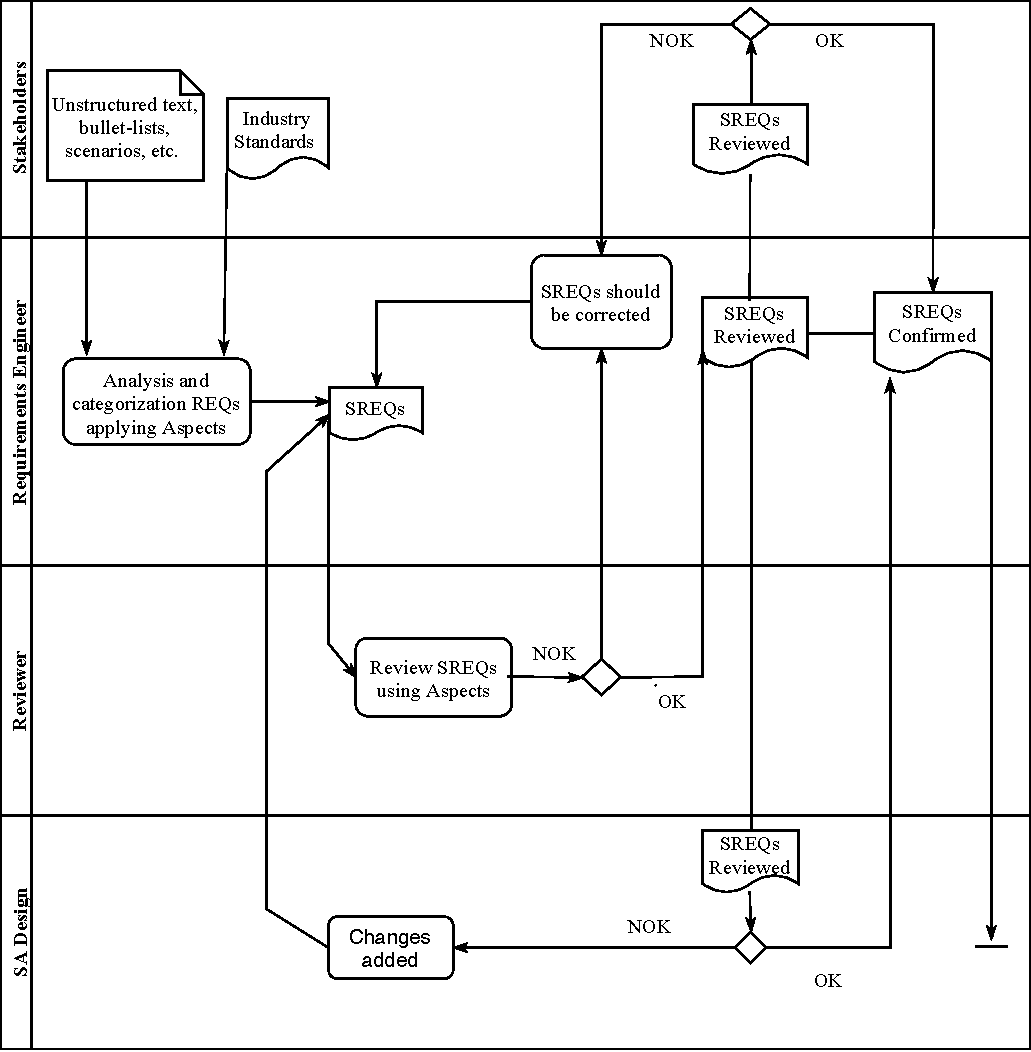
\includegraphics[width=3.5in]{wf_Aspects.pdf}
\caption{Work flow supported by \textit{aspects} during requirements analysis and review}
\label{fig:fig_review}
\end{figure}

The process divided into parts by roles. Here the main roles are a requirements engineer (REer), a reviewer and developers; the responsibilities of Stakeholders role can be delegated to requirements engineer or reviewer \cite{17MiniDuide}.  

\textit{1. Stakeholders.}

Stakeholders very often provide requirements in a textual form, which has no structure or can consist of bulleted lists, long sentences with specification and etc. Example of such “raw” requirement: 

\textit{“The input for the component shall be Z number of latency limits, assigned to the ring buffers, with allowed range [Xms; Yms].”}  

Requirements is provided to requirements engineer for further analysis. AF3 supports requirements in textual format and text of requirements can be imported into AutoFOCUS 3. 

\textit{2. Requirements engineer.}

\textit{Aspects} can be applied to system requirements from initial stage of the development, from requirements elicitation. The requirements engineer should analyze and structure these requirements accordingly, so that in future it will take less effort to translate an inferred System Requirements (SREQs) into appropriate High Level Requirements (HLR) and Low Level Requirements (LLR) for system design.

For this project eight aspects have been implemented in AutoFOCUS 3, which represent diversity of requirements' objectives (Figure~\ref{fig:fig_aspects}).

\begin{itemize}
\item	\textit{Timing aspect} - the requirement refers to timing constraints
\item	\textit{Signal aspect} - the requirement defines a signal, its type and its range
\item	\textit{Parameter definition aspect} - the requirement defines a parametric value. This allows to reused other requirements by changing the value of the parameter
\item\textit{Safety level aspect} - the requirement defines a safety level of the system
\item	\textit{Mode aspect}- the requirement defines an operational mode of the system
\item	\textit{Design choice aspect} - the requirement was derived from a design choice of the software developer
\item	\textit{Functional aspect}- the requirement specifies a particular behavior by relating inputs and outputs
\item	\textit{Temporal property aspect} - the requirement defines a property expressed by temporal patterns
\end{itemize}

\begin{figure}[!t]
\centering
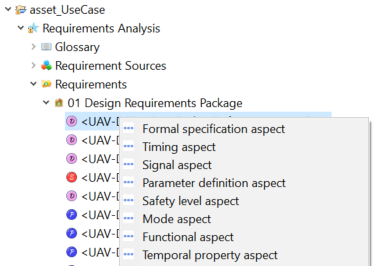
\includegraphics[width=2in]{asset_aspects.png}
\caption{List of \textit{aspects} in AutoFOCUS 3}
\label{fig:fig_aspects}
\end{figure}

Depending on characteristics of the considered requirement, the appropriate \textit{aspect }or set of \textit{aspects} can be applied to it. The number of applied aspects can indicate about complexity of the requirement exposing that too many responsibilities endow on it. Such requirement should be revised for further transformation (e.g. splitting into several less complex requirements). For instance, to structure this system requirement the following \textit{aspects} can be applied to it: a signal \textit{aspect}, a parameter \textit{aspect}, timing \textit{aspect} and temporal aspect as well. Therefore, the system requirement content is not changed, but the main characteristics of this statement are defined. The number of attached \textit{aspects} shows, that the requirement can be divided into several requirements matching to the categorization. In this case, the requirement can be splitted into the following list:
\begin{itemize}
 \item “the input for the component shall be Z number of latency limit” – \textit{signal} and \textit{parameter aspects};
 \item “latency limits are assigned to the ring buffers” - \textit{parameter aspect};
 \item “latency limits has allowed range [Xms; Yms] ” – \textit{parameter} and \textit{temporal aspects};
\end{itemize}

Now, these categorized requirements can be revised.

\textit{3. Reviewer.}

In the ASSET project this procedure required a manual check according to industry standard DO-178C \cite{7DO-178C}. 

Every aspect provides to a reviewer a set of instruments which supports a revision process, such as check-lists defined for every aspect. Review process is maintained by check-lists inferred form the aspects. These check-lists aim to more accurate and precise requirements inspection and bring about various methods for analysis. In AF3 these check-lists is going to be implemented as a semi-automatized feature to reinforce requirements review.

The reviewer checks provided SREQs, which are still in the text form with aspects attached to them. 
Working with aspects artifact a reviewer can examine SREQs for the following points:
\begin{itemize}
	\item if the \textit{aspects} applied for every requirement,
  \item if the combination of \textit{aspects} matches to the scope of requirements and
	\item if all check-lists give successful outcomes.
\end{itemize}

%According to different Aspects may be taken in account diverse analysis methods and review activities during requirements examination. Furthermore, every Aspect provides a checklist specified according to a represented requirement category, which gives an ability to write requirements and review them in one tool, instead of using different tools for every activity. In AutoFOCUS 3 checklists implemented as automatized.

In positive  case, the SREQs can be provided further as an input to System Architecture design for a development team and/or to stakeholders for next consideration. SREQs is a textual artifact with attached aspects. Therefore, stakeholders work again with a document of text requirements.
In case the check of SREQs fails, a reviewer can re-apply aspects to requirements and send back to REer for repeated analysis and correction. REer now have attached aspects as “hints”, so that he/she can clearly understand the nature of the correction in SREQs and restart the requirements analysis again.

\textit{4. Developers}

For developers use there exists a \textit{“Design Choice” aspect}, so that they can indicate new changes in requirements coming from their side and by that initiate a revision procedure again.

After checking succeeds and HLR have been also conformed by stakeholders, the procedure with the aspects application can be repeated again in order to derive HLR and LLR and then a new review starts.

\subsection{Results:}
\textit{Aspects} concept implementation in AF3 reveals that all described activities can be performed in one tool. It gives an advantage with keeping traceability between all levels of requirements from system requirements to HLR and LLR as well as between requirements and system design, which is critical for avionics system. The approach supports traceability between requirements on all stages of development. Furthermore, \textit{aspects} concept incarnate a common instrument for all roles involved in requirements engineering process and narrow a gap between requirements engineers, reviewers and developers by formalizing requirements and holding up a guidance for these roles.

Additionally, flexibility of categorization-based concept allows to avoid problems caused by changes of requirements during a whole system life cycle. The aspect method leaves a possibility for ``late'' amendments and modifications in requirements.

This use case has been validated in an industrial project (ASSET) conducted by Airbus with Fortiss for developing a component for avionics system in AutoFOCUS 3. 


%The following use cases will be discussed for the Aspects better explanation:

%1.	Use Case provides an example of requirements and shows how the Aspects concept can be applied for structuring requirements. This Use case can be validated by empirical experiments considered to be conducted further within this research.
%2.	Use Case of avionics component development applying the Aspects. This use case shows how the Aspects concept supports a process of requirements review. The use case was approved within industrial project (ASSET) conduct-ed by Aerobus with Fortiss.
%3.	Use Case “Beyond AF3” is an inner project of Fortiss, which validate a general nature of the Aspects concept. In other words, it demonstrates independency of the Aspects concept from a precise chain of tools.


%Commonly, a development process starts from the requirements elicitation mostly as text and analysis. AF3 supports requirements in textual format and provide the author to choose which Aspect is relevant to the considered requirement.



%user to compose a set of appropriate categories with different granularity of any category in the set.The Aspects compose different types with diverse granularity.

%\subsection {Use Case1: Requirements categorization using the Aspects.}
%
%The process of requirements reviewing is described further in Use Case 2.
%
%\subsection {Use Case 2: Requirements engineering and reviewing with use of the Aspects.}
%There is a description of the work flow supported by Aspects during requirements analysis and review. This method was realized in AutoFOCUS 3 within ASSET project developing a component for avionics system (Figure 2).
%\begin{figure}[!t]
%\centering
%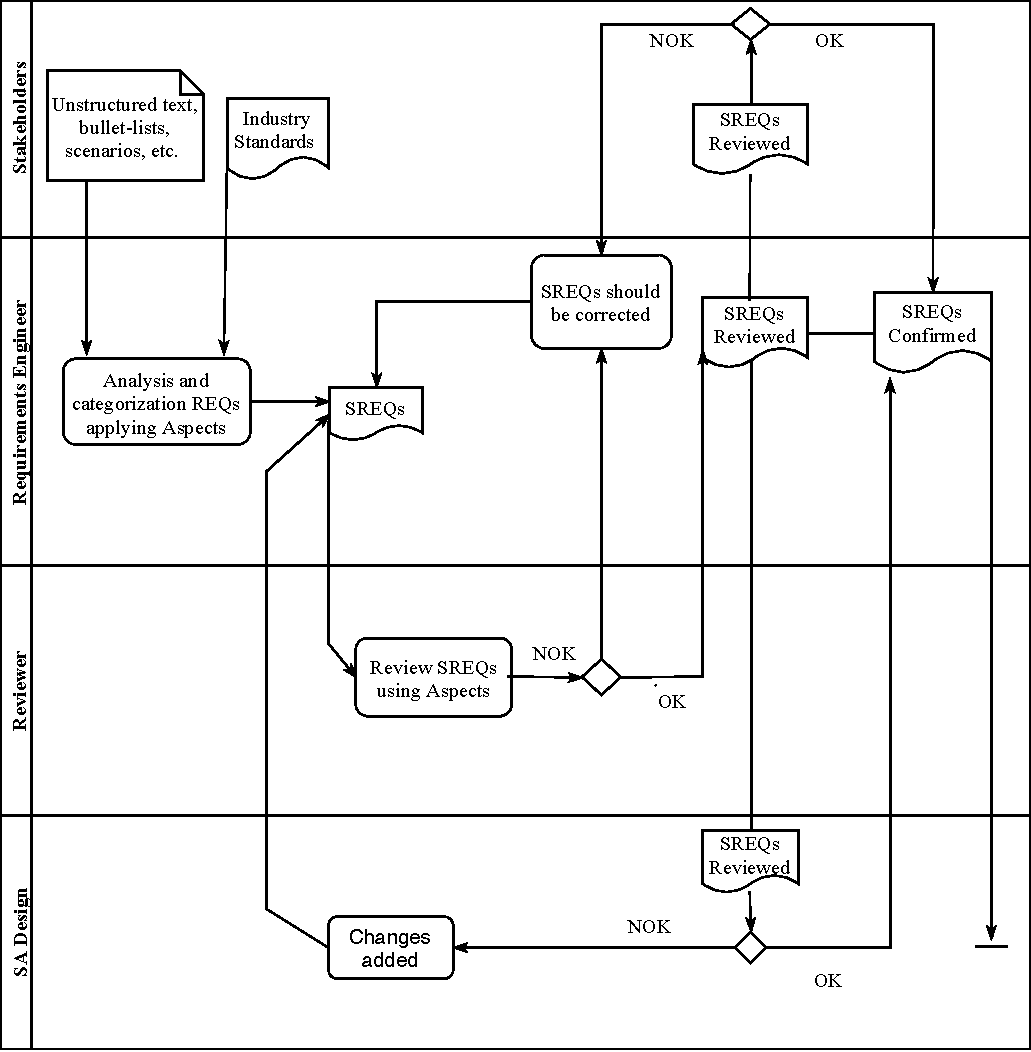
\includegraphics[width=2.5in]{wf_Aspects.pdf}
%\caption{Work flow supported by Aspects during requirements analysis and review.}
%\label{fig_review}
%\end{figure}
%
%The process divided into parts by roles. The main roles here are a requirements engineer (REer) and a reviewer; the responsibilities of roles Stakeholders and SA design can be delegated to the main roles [17].  

%The Aspects can be applied to system requirements from initial stage of the development, from system requirements (SRs) elicitation (see use case1). SRs  analyzing and structuring requirements by the Aspects transforms into HLRs. Now HLRs can be provided to a reviewer for checking. 
%The reviewer checks manually the HLRs, which are still in the text form and the Aspects attached to them. In context of aspects, a reviewer can examine HLRs for the following points:
%•	if the Aspects applied for every requirement and 
%•	if the combination of Aspects matches to the HLRs.

%Review process is maintained by check-lists inferred form the Aspects (every aspect has its own check-list). In AF3 these check-lists implemented as a semi-automatized feature to reinforce requirements review.

%In positive  case, the HLRs can be provided further to SA design team and/or to stakeholders for next consideration. HLRs is a textual artifact with attached aspects, which sup-ports the HLRs structure. Therefore, stakeholders work again with a document of text requirements.
%In case the check of HLRs fails, a reviewer re-applies the Aspects to HLRs and re-structures them and sends back to REer for repeated analysis and correction. REer now have a “hints” in a form of aspects structure attached to HLRs by a reviewer, so that he/she can clearly understand the nature of the correction in HLRs and restart the requirements analysis again.

%For Developers use there exists a “Design Choice” aspect, so that they can indicate a new changes in requirements coming from their side and by that initiate a revision procedure again.
%
%After this procedure, the HLRs confirmed and can be as an input to SA design process and to further LLRs. The procedure with LLRs starts with the analysis process and transforming the structure of the requirements applying the Aspects; and all procedure described above repeats for LLRs.
%The Aspect supports traceability between requirements on all stages of development. Furthermore, the Aspects appears here as a common instrument for all roles within requirements engineering and review processes guiding them through the work flow.

%The Aspects concept implementation in AF3 reveals, that all described activities can be performed in the same tool. It gives an advantage with keeping traceability between all levels of requirements from SR to HLR and LLR as well as between requirements and system design, which is critical for avionics.

